\documentclass[conference]{IEEEtran}

% ========= 日本語対応(LuaLaTeX推奨) =========
\usepackage{luatexja}
\usepackage{luatexja-fontspec}
\setmainjfont{HaranoAjiMincho}
\setsansjfont{HaranoAjiGothic}

% ========= 一般パッケージ =========
\usepackage{amsmath,amssymb}
\usepackage{graphicx}
\usepackage{booktabs}
\usepackage{array}
\usepackage{url}
\usepackage[hidelinks]{hyperref}
\usepackage{cite}
\usepackage{siunitx}
\sisetup{
  detect-all = true,
  per-mode   = symbol,
  range-phrase = --,
  product-units = single
}
\let\meter\metre

% ========= 図・グラフ =========
\usepackage{tikz}
\usetikzlibrary{arrows.meta,decorations.pathreplacing,calc,patterns}
\usepackage{pgfplots}
\pgfplotsset{compat=1.18}

% ========= タイトル =========
\title{セイコーエプソン酒田Fab 8インチライン立ち上げ\\
DRAM技術導入から量産化そしてその役割(1997--2001)}

\author{%
  \IEEEauthorblockN{三溝 真一 (Shinichi Samizo)}%
  \IEEEauthorblockA{独立系半導体研究者(元セイコーエプソン)\\%
  Independent Semiconductor Researcher (ex-Seiko Epson)\\%
  Email: \href{mailto:shin3t72@gmail.com}{shin3t72@gmail.com}\\%
  GitHub: \url{https://github.com/Samizo-AITL}}%
}

\begin{document}
\maketitle

\begin{abstract}
\textbf{(日本語)}\\
本稿は,1997--2001年にセイコーエプソン酒田事業所が
三菱電機からの技術移管により
\SI{0.5}{\micro\meter} $\rightarrow$ \SI{0.35}{\micro\meter} $\rightarrow$ \SI{0.25}{\micro\meter}
のDRAMプロセスを短期間で立ち上げ,量産化した過程を整理する。
主眼はDRAM導入・量産化であり,Pause/Disturb Refresh不良の解析と対策,歩留まり推移,
および\emph{量産インフラとしての役割}を明確化する。
その後,社内設計によるVSRAM開発やNANYA 0.18\,$\mu$m評価を経て,
DRAMの役割を終えた後に,酒田Fabが社内外のロジック/高耐圧混載CMOS展開に
寄与した戦略的意義を振り返る。\\[0.7ex]

\textbf{(English)}\\
This paper documents the introduction and mass production of DRAM processes
(\SI{0.5}{\micro\meter} $\rightarrow$ \SI{0.35}{\micro\meter} $\rightarrow$ \SI{0.25}{\micro\meter})
transferred to Seiko Epson's Sakata Fab (1997--2001).
We focus on DRAM-specific failure analyses (Pause/Disturb Refresh), countermeasures, and yield evolution,
clarifying the DRAM line's role as manufacturing infrastructure.
Later, VSRAM development and evaluation of a NANYA 0.18\,$\mu$m process marked the end of memory products,
while the acquired process infrastructure supported Epson's strategies in logic, SoC, and high-voltage mixed-CMOS.
\end{abstract}

\begin{IEEEkeywords}
DRAM, VSRAM/PSRAM, \SI{0.25}{\micro\meter} process, retention failure, disturb failure, Sakata Fab, technology transfer, SCF
\end{IEEEkeywords}

\section{序論}
1997年,当時の半導体産業は \textit{Windows 95} の世界的普及や
Intel Pentium II の登場を背景に急成長局面にあった。
パソコンの性能向上と普及拡大が同時に進み,
メモリ容量・処理性能に対する市場要求は急速に高まっていた。

製造技術面では,8インチウェーハラインの整備と
\SI{0.35}{\micro\meter} 世代プロセスへの移行が加速し,
DRAMおよびロジックLSI分野における国際競争が激化していた。

セイコーエプソンは山形県酒田市に新設した 8インチFabにおいて,
三菱電機からの技術移管を通じて
\SI{0.5}{\micro\meter} $\rightarrow$ \SI{0.35}{\micro\meter} $\rightarrow$ \SI{0.25}{\micro\meter}
の三世代DRAMプロセスを短期間で習得し量産化に至った。

本稿では,このDRAM技術導入と量産化の過程を主軸として,
Pause/Disturb Refresh不良の解析と対策,歩留まり推移を整理する。
さらに,酒田FabのDRAM量産ラインが,
その後のロジック/高耐圧混載CMOS開発の\emph{インフラ}として果たした役割を振り返る。

\section{第1章:\texorpdfstring{\SI{0.5}{\micro\meter}}{0.5μm} と \texorpdfstring{\SI{0.35}{\micro\meter}}{0.35μm} 世代の立ち上げ}

\subsection{\SI{0.5}{\micro\meter} 16M DRAM}
酒田Fabの最初の量産は \SI{0.5}{\micro\meter} 世代16M DRAMであった。
熊本Fabで確立されたプロセスを忠実に移管したため,
装置親和性が高く立ち上げは極めてスムーズであった。

\begin{itemize}
  \item 熊本Fab実績の完全移植(装置・順序・ケミカル・搬送条件まで忠実)
  \item 初期歩留まりから安定して高水準
  \item 短期間で量産KPI域に到達
\end{itemize}

この成功により,酒田Fabは「量産能力を有する新拠点」であることを実証し,
次世代プロセス挑戦の足場を得た。

\subsection{\SI{0.35}{\micro\meter} 64M DRAM:洗浄フロー差異と「鏡写し」}
次の挑戦は \SI{0.35}{\micro\meter} 世代の64M DRAMであった。

\subsubsection*{初期の困難}
1997年秋,試作ロット30ロット超を投入したが,
SEM観察すら困難なほどのパターン崩れが頻発。
熊本Fabでは安定していた条件が再現できず,
現場は停滞と混乱に陥った。

\subsubsection*{原因究明}
徹底調査の結果,原因は「洗浄フロー差異」であると判明。  
\begin{itemize}
  \item 熊本:硫酸過水 $\rightarrow$ アンモニア過水 $\rightarrow$ 塩酸過水(3段)
  \item 酒田:アンモニア過水 $\rightarrow$ 塩酸過水(前段省略)
\end{itemize}

この差異が表面状態を変化させ,
後段プラズマ処理と干渉して膜厚ばらつきを拡大,
パターン形状崩壊を誘発していた。

\subsubsection*{解決:完全「鏡写し」}
最終解決策は,熊本条件の一切の省略なし移植。
洗浄工程を含む全フローを完全に鏡写しした結果,
形状不良は消失し量産移行に成功。
「先端プロセス移管では二次因子も省略不可」というFab全体の教訓となった。

\subsection{小括}
\begin{itemize}
  \item \SI{0.5}{\micro\meter}:熊本Fab実績の完全移管で安定立ち上げ。
  \item \SI{0.35}{\micro\meter}:洗浄フロー省略が致命的要因。
  \item 解決は「鏡写し」による完全移管。
\end{itemize}
これらの経験が,次世代 \SI{0.25}{\micro\meter} プロセス立ち上げの基盤となった。

\section{第2章:\texorpdfstring{\SI{0.25}{\micro\meter}}{0.25μm} 世代64M DRAMの立ち上げ}

\subsection{SCF方式と初期歩留まり}
1998年,酒田Fabは \SI{0.25}{\micro\meter} 世代64M DRAMに挑戦した。
ここでも三菱電機が確立していた \emph{Short Cycle Feedback (SCF)} 方式を導入。
工程を短サイクルで止め,SEM観察・電気評価を繰り返しながら条件修正する方式である。

\begin{enumerate}
  \item 熊本からの条件を流動票へ展開
  \item 工程ごとに形式ロットを途中止めし形状観察
  \item SEM・電気評価フィードバックで逐次修正
  \item 本番ロットで信頼性確認
\end{enumerate}

その結果,初期歩留まり65\%という極めて高い値を達成。
従来の新世代DRAM初期値(20--30\%)を大きく上回った。

\subsection{保持時間モデルと不良モード解析}
不良は主に \emph{Pause Refresh Fail} に集中した。
リフレッシュを停止しセル保持を確認する試験で,
32ms $\rightarrow$ 64ms $\rightarrow$ 128ms と条件を厳しくすると,
ランダムに単ビット不良が発生(Fig.~\ref{fig:failmap})。

保持時間は
\[
\tau = \frac{C_{\mathrm{cell}} V_{\mathrm{cell}}}{I_{\mathrm{leak}}}
\]
で与えられ,設計値 $C_{\mathrm{cell}}, V_{\mathrm{cell}}$ に問題はなく,
リーク電流 $I_{\mathrm{leak}}$ が支配的要因であると判明した。

レイアウト欠陥は否定され,主因は \emph{拡散層ジャンクションリーク}。
フェイルマップ再現性から,プロセス条件起因の系統的不良であることが確定した。

\begin{figure}[t]
\centering
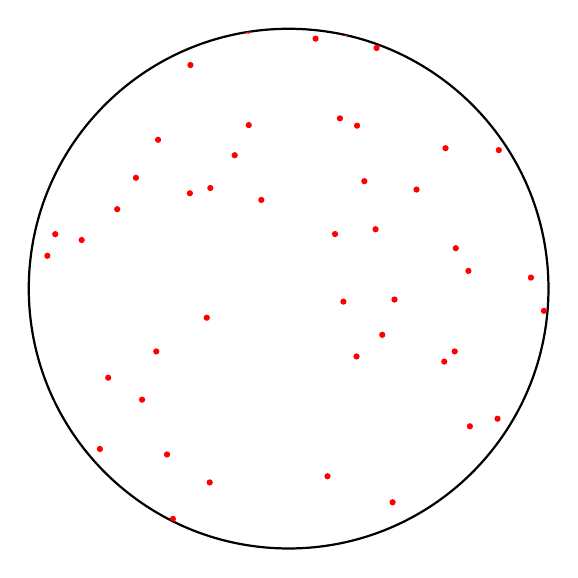
\begin{tikzpicture}[scale=0.22]
  \def\R{15}
  \draw[thick] (0,0) circle (\R);
  \begin{scope}
    \clip (0,0) circle (\R);
    \foreach \i in {1,...,60}{
      \pgfmathsetmacro{\xx}{(rnd*2-1)*\R}
      \pgfmathsetmacro{\yy}{(rnd*2-1)*\R}
      \fill[red] (\xx,\yy) circle (0.18);
    }
  \end{scope}
\end{tikzpicture}
\caption{Pause Refresh Fail のフェイルマップ例}
\label{fig:failmap}
\end{figure}

\subsection{プラズマダメージ仮説}
ジャンクションリーク増大の背景にはプラズマダメージが疑われた。
\begin{itemize}
  \item ゲートエッチ後酸化膜露出時
  \item LDD工程での繰返しアッシング
\end{itemize}
O$_2$プラズマが界面欠陥を生成し,熱励起キャリアリークを助長すると推定。

\subsection{対策と効果}
根本対策は「O$_2$アッシング剥離 $\rightarrow$ 硫酸ウェット剥離」への全面切替。
プラズマ曝露をゼロ化することでリークを抑制。

\begin{table}[h]
  \centering
  \caption{レジスト剥離フロー切替}
  \label{tab:resist}
  \begin{tabular}{lll}
    \toprule
    & 従来 & 対策後 \\
    \midrule
    剥離方式 & O$_2$アッシング & 硫酸ウェット \\
    主効果 & プラズマ曝露 & 界面欠陥防止 \\
    歩留まり & 65\% & 80\%台後半 \\
    \bottomrule
  \end{tabular}
\end{table}

対策後,Pause不良は激減し,歩留まりは80\%台後半に安定(Fig.~\ref{fig:yield25})。

\begin{figure}[t]
\centering
\begin{tikzpicture}
\begin{axis}[
  width=\linewidth, height=5cm,
  ymin=0, ymax=100,
  ylabel={歩留まり(\%)},
  symbolic x coords={0.35\,μm,0.25\,μm},
  xtick=data,
  grid=both
]
  \addplot+[mark=*] coordinates {(0.35\,μm,20) (0.25\,μm,65)};
  \addlegendentry{初期}
  \addplot+[mark=square*] coordinates {(0.35\,μm,86) (0.25\,μm,88)};
  \addlegendentry{改善後}
\end{axis}
\end{tikzpicture}
\caption{酒田Fab:世代別歩留まり推移}
\label{fig:yield25}
\end{figure}

\subsection{小括}
\begin{itemize}
  \item SCF方式により迅速な条件整備と65\%初期歩留まりを達成。
  \item 不良主因はジャンクションリーク,プラズマダメージが背景。
  \item 硫酸ウェット剥離への切替で歩留まりは80\%台後半に改善。
\end{itemize}
この知見は「表面処理・プラズマ影響を軽視不可」という教訓を残し,
Fab自前化の礎となった。

\section{第3章:VSRAM(2001年)— Pause/Disturb対策と歩留まり改善}

\subsection{開発背景と初期状況}
2001年,当時の携帯電話市場では「世界初のカメラ付き携帯」の投入が計画され,
低消費電力かつ高温(90$^\circ$C)動作保証のメモリが求められた。
酒田Fabは \SI{0.25}{\micro\meter} DRAMプロセスを流用し,
内部リフレッシュ回路を付加して \emph{VSRAM(疑似SRAM)} を開発。

しかし初期量産歩留まりは約30\%に留まり,
タイムリミットを優先して「低歩留まりで量産開始」という厳しい判断が下された。
筆者はこの時点から改善担当として参画した。

\subsection{顕在化した不良モード}
VSRAM特有の不良は以下の2種類であった:
\begin{itemize}
  \item \textbf{Pause Refresh Fail}:リフレッシュ停止時にセル保持が崩壊。
  \item \textbf{Disturb Refresh Fail}:隣接ワードライン電圧干渉による誤反転。
\end{itemize}

Pauseは従来から存在したが,Disturbはモバイル用途での長リフレッシュ+高温条件で顕在化。

\subsection{物理的要因}
Pauseの主因はジャンクションリーク。
保持時間モデル
\[
\tau = \frac{C_{\mathrm{cell}} V_{\mathrm{cell}}}{I_{\mathrm{leak}}}
\]
において $I_{\mathrm{leak}}$ 増大で $\tau$ が短縮。
温度上昇で $I_{\mathrm{junc}}$ が指数的に増加(Fig.~\ref{fig:pause})。

Disturbは短チャネル効果(SCE)が原因。
CDが短いほど $I_{\mathrm{off}}$ が急増し,
高温でさらに顕著(Fig.~\ref{fig:disturb})。

\begin{figure}[t]
\centering
\begin{tikzpicture}
\begin{axis}[
  width=\linewidth, height=5cm,
  xlabel={温度 [$^\circ$C]}, ylabel={$I_{\mathrm{junc}}$ (相対)},
  ymode=log, ymin=1e-2, ymax=1e2, xmin=25, xmax=100
]
  \addplot+[mark=*] coordinates {(25,0.02)(40,0.06)(60,0.3)(80,1.6)(90,3.2)(100,6.0)};
  \addlegendentry{$V_{bs}=-1$V}
  \addplot+[mark=square*] coordinates {(25,0.01)(40,0.03)(60,0.12)(80,0.45)(90,0.9)(100,1.8)};
  \addlegendentry{$V_{bs}=-3$V}
\end{axis}
\end{tikzpicture}
\caption{Pause Refresh:温度依存とバックバイアス効果}
\label{fig:pause}
\end{figure}

\begin{figure}[t]
\centering
\begin{tikzpicture}
\begin{axis}[
  width=\linewidth, height=5cm,
  xlabel={温度 [$^\circ$C]}, ylabel={$I_{\mathrm{off}}$ (相対)},
  ymode=log, ymin=1e-3, ymax=1e1, xmin=25, xmax=100
]
  \addplot+[mark=triangle*] coordinates {(25,0.004)(40,0.01)(60,0.05)(80,0.22)(90,0.45)(100,0.9)};
  \addlegendentry{CD=0.25μm}
  \addplot+[mark=*] coordinates {(25,0.01)(40,0.03)(60,0.15)(80,0.7)(90,1.4)(100,2.8)};
  \addlegendentry{CD=0.20μm}
\end{axis}
\end{tikzpicture}
\caption{Disturb Refresh:短チャネル効果と温度依存}
\label{fig:disturb}
\end{figure}

\subsection{対策と実装}
\begin{itemize}
  \item Pause対策:
    \begin{itemize}
      \item HF洗浄回数を最小化し,SNコンタクトリークを抑制。
      \item バックバイアス強化($-1$V $\rightarrow$ $-3$V)でジャンクションリークを低減。
    \end{itemize}
  \item Disturb対策:
    \begin{itemize}
      \item ゲートCD管理を徹底。
      \item バックバイアス強化でしきい値電圧上昇。
      \item チャネルドーピング増加でセル反転耐性を確保。
    \end{itemize}
\end{itemize}

\begin{table}[t]
\centering
\caption{Pause/Disturb不良への主対策}
\begin{tabular}{lll}
\toprule
不良 & 主因 & 対策 \\
\midrule
Pause & 接合リーク & HF制御,$V_{bs}$強化 \\
Disturb & 短チャネル効果 & CD管理,ドーピング,$V_{bs}$強化 \\
\bottomrule
\end{tabular}
\end{table}

\subsection{効果と歩留まり推移}
Pause/Disturbは大幅に減少。
歩留まりは初期30\% $\rightarrow$ 80\%台へ改善し,
量産に耐える水準に到達。

\subsection{小括}
\begin{itemize}
  \item モバイル要求(低消費・90$^\circ$C保証)がPause/Disturb不良を顕在化させた。
  \item HF洗浄制御,バックバイアス強化,ゲート寸法管理などにより,
        歩留まりは30\%から80\%台へ大幅に改善。
  \item VSRAMは,酒田FabにおけるDRAM派生メモリ開発の集大成として,
        厳しい市場要求に応えつつ量産を実現した。
\end{itemize}

\section{第4章:\texorpdfstring{\SI{0.18}{\micro\meter}}{0.18μm} トレンチ系の評価と断念}

\subsection{評価対象と背景}
VSRAM立ち上げ後,次世代候補として
台湾NANYA社の \SI{0.18}{\micro\meter} DRAMプロセスを利用した
VSRAM試作評価が検討された。
NANYAは東芝と技術提携しており,
\emph{トレンチキャパシタ方式}を基盤とするプロセスを供与していた。

目的は,\SI{0.25}{\micro\meter} DRAM流用VSRAMの後継として,
さらに高密度・低消費・高温動作保証を満たすモバイル向けメモリを実現することにあった。

\subsection{技術的特徴}
\begin{itemize}
  \item \textbf{キャパシタ構造}:スタック型に対し,面積効率の高いトレンチ型を採用。
  \item \textbf{動作仕様}:標準DRAM同様に80$^\circ$C保証は可能だが,
        モバイル用途必須の90$^\circ$C保証には余裕がなかった。
\end{itemize}

\subsection{課題の顕在化}
試作評価の結果,90$^\circ$C条件下で以下の不良が顕著となった:
\begin{itemize}
  \item Pause Refresh Fail:セル保持時間不足。
  \item Disturb Refresh Fail:高温条件で誤反転が増加。
  \item 高温リーク:pn接合リークが著しく増大。
\end{itemize}

\begin{figure}[t]
\centering
% ==== Stack Cross-section ====
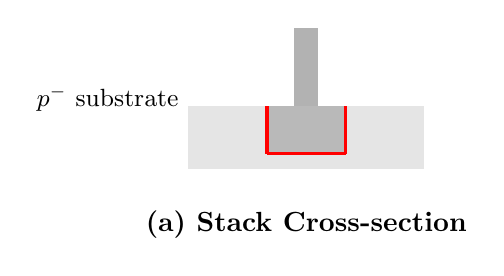
\begin{tikzpicture}[x=1cm,y=1cm]
  % substrate
  \fill[gray!20] (-1.5,0) rectangle (1.5,-0.8);
  \node[anchor=east] at (-1.5,0.1) {\small $p^-$ substrate};

  % n+ diffusion
  \fill[gray!55] (-0.5,0) rectangle (0.5,-0.6);

  % electrode
  \fill[black!30] (-0.15,0) rectangle (0.15,1.0);

  % pn junction lines
  \draw[red,very thick] (-0.5,0) -- (-0.5,-0.6);
  \draw[red,very thick] (0.5,0) -- (0.5,-0.6);
  \draw[red,very thick] (-0.5,-0.6) -- (0.5,-0.6);

  \node[anchor=north] at (0,-1.2) {\bfseries (a) Stack Cross-section};
\end{tikzpicture}

\vspace{1.0em}

% ==== Trench Cross-section ====
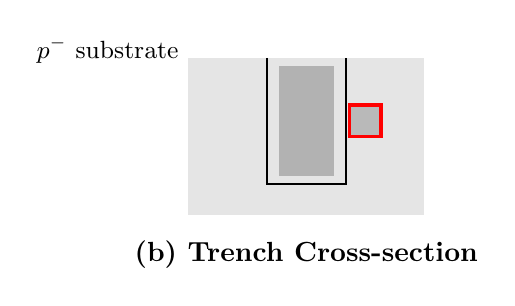
\begin{tikzpicture}[x=1cm,y=1cm]
  % substrate
  \fill[gray!20] (-1.5,0) rectangle (1.5,-2.0);
  \node[anchor=east] at (-1.5,0.1) {\small $p^-$ substrate};

  % trench cavity
  \draw[black,thick] (-0.5,0) -- (-0.5,-1.6) -- (0.5,-1.6) -- (0.5,0);

  % electrode inside trench
  \fill[black!30] (-0.35,-0.1) rectangle (0.35,-1.5);

  % buried strap diffusion
  \fill[gray!55] (0.55,-0.6) rectangle (0.95,-1.0);

  % pn junction highlight
  \draw[red,very thick] (0.55,-0.6) rectangle (0.95,-1.0);

  \node[anchor=north] at (0,-2.2) {\bfseries (b) Trench Cross-section};
\end{tikzpicture}

\caption{Stack型とTrench型キャパシタ構造比較。
Stackは接合周辺長が限定的,Trenchはburied strap起点で周辺長が増大。}
\label{fig:stack_trench}
\end{figure}

\subsection{リーク増大の構造的起因}
Fig.~\ref{fig:stack_trench} に示すように,
Stack型では接合は拡散層の側壁と底面のみであり,周辺長は短い。
一方,Trench型では \emph{buried strap} 周囲に局所接合が形成され,
セル列構造により周辺長が大幅に増加する。
この構造差が高温リークを顕著化させた。

\begin{figure}[t]
\centering
\begin{tikzpicture}
\begin{axis}[
  width=\linewidth, height=6cm,
  xlabel={ジャンクション面積(相対)}, ylabel={$I_{\mathrm{junc}}$(相対)},
  xmin=0.5, xmax=2.5, ymin=0, ymax=3,
  grid=both,
  legend style={at={(0.5,-0.22)},anchor=north,draw=none,fill=none},
  clip=false
]
  \addplot+[mark=square*] coordinates {
    (0.5,0.25) (1.0,0.5) (1.5,0.8) (2.0,1.1) (2.5,1.4)
  };
  \addlegendentry{80$^\circ$C}
  \addplot+[mark=*] coordinates {
    (0.5,0.5) (1.0,1.0) (1.5,1.6) (2.0,2.2) (2.5,2.9)
  };
  \addlegendentry{90$^\circ$C}
\end{axis}
\end{tikzpicture}
\caption{トレンチ型セルにおけるジャンクションリークの面積依存性。
高温条件では増加率がさらに大きい。}
\label{fig:trench_leak}
\end{figure}

\subsection{評価結果と戦略判断}
NANYA \SI{0.18}{\micro\meter} トレンチプロセスは,
90$^\circ$C保証を満たせず,次世代VSRAMとして不適と判断。
このため酒田FabでのDRAM派生製品開発は終息し,
経営資源は液晶ドライバー向け高耐圧混載CMOSに集中した。

\subsection{小括}
\begin{itemize}
  \item トレンチ方式は高密度化に有利だが,高温リーク増大でモバイル仕様に不適。
  \item 90$^\circ$C保証を満たせず,次世代VSRAMは断念。
  \item 以後は液晶ドライバーを中心とする高耐圧混載CMOSに軸足を移した。
\end{itemize}

\section{結論}

本研究では,1997年から2001年にかけて酒田Fabで行われた
DRAM技術導入とその戦略的展開を,筆者の現場経験に基づいて整理した。

\begin{itemize}
  \item \textbf{第1章}:\SI{0.5}{\micro\meter} 世代16M DRAMは熊本Fabプロセスの忠実移管で安定立ち上げ。
        \SI{0.35}{\micro\meter} 世代64M DRAMでは洗浄フロー差異が原因で大規模不良が発生したが,
        熊本条件の完全「鏡写し」によって解決し,移管プロセスにおける
        「二次因子も含めて省略不可」という原則がFab全体の教訓となった。
  \item \textbf{第2章}:\SI{0.25}{\micro\meter} 世代64M DRAMはSCF方式により短期間で量産条件を整備。
        初期歩留まり65\%からスタートし,不良解析でジャンクションリークを主因と特定。
        O$_2$アッシングを硫酸ウェット剥離に全面切替することで
        歩留まりは80\%台後半に改善した。
  \item \textbf{第3章}:VSRAMではモバイル要求(低消費・90$^\circ$C保証)がPause/Disturb不良を顕在化させた。
        HF洗浄回数の最小化,バックバイアス強化,ゲート寸法管理により,
        歩留まりは30\%から80\%台に大幅改善。酒田FabにおけるDRAM派生メモリ開発の集大成となった。
  \item \textbf{第4章}:NANYA \SI{0.18}{\micro\meter} トレンチプロセス評価では,
        高温リークの増大により90$^\circ$C保証を満たせず,次世代VSRAMは断念。
        この時点でメモリ派生製品の展開は終息へ向かい,
        経営資源は液晶ドライバー用高耐圧混載CMOSに集中した。
\end{itemize}

\noindent
以上を総括すると,酒田FabにおけるDRAM導入は「事業の最終目的」ではなく,
\textbf{最先端プロセス知見を獲得するための手段}であった。  
DRAM量産を通じて習得した表面処理・接合リーク制御・CD管理の知見は,
その後の液晶ドライバーや高耐圧混載CMOS開発に直結し,
エプソンのコア事業を支える技術基盤となった。

さらに,この知見はVSRAMと並行して,外販ファンドリ(Xilinx等)や
社内SoC/マイコン製品開発へも展開されており,
\textbf{DRAM導入を起点とする複線的な技術・事業展開戦略}が形成された。  

すなわち,酒田FabのDRAM導入の歴史的意義は,
単なるDRAM製造にとどまらず,
\emph{先端ロジック/混載CMOS/ディスプレイドライバー/SoC/マイコン/ファンドリビジネス}といった
広範な事業基盤への並行展開を可能にした点にある。

\section*{参考文献}
\begin{thebibliography}{00}
\bibitem{sze2006psd}
S.~M.~Sze and K.~K.~Ng, \emph{Physics of Semiconductor Devices}, 3rd ed., Wiley, 2006.

\bibitem{tanaka1996dramtrends}
T.~Tanaka et al., ``Trends and Challenges in DRAM Scaling,'' \emph{IEEE J. Solid-State Circuits}, vol.~31, no.~11, pp.~1615--1624, 1996.

\bibitem{rizzoli2000retention}
L.~Rizzoli et al., ``Retention and Disturb Characterization in 0.25 Micron DRAM,'' in \emph{Proc. Int. Test Conf.}, 2000.

\bibitem{okhonin1998retention}
S.~Okhonin et al., ``Retention Time and Junction Leakage in Deep Submicron DRAM,'' in \emph{IEDM Tech. Dig.}, pp.~549--552, 1998.

\bibitem{wong1999dram}
H.-S.~P.~Wong, ``Technology and Device Scaling for DRAM,'' \emph{IBM J. Res. Dev.}, vol.~43, no.~1–2, pp.~133--168, 1999.

\bibitem{chang1994plasma}
C.~Chang and S.~C.~Lee, ``Plasma-Induced Damage on Gate Oxides,'' \emph{J. Electrochem. Soc.}, vol.~141, no.~9, pp.~2512--2517, 1994.

\bibitem{mosys2001}
MoSys Inc., ``1T-SRAM Technology Overview,'' White Paper, 2001.

\bibitem{kim2002psram}
J.~Kim et al., ``Low Power Refresh Schemes for Mobile DRAM/PSRAM,'' in \emph{Symp. on VLSI Circuits}, pp.~190--193, 2002.

\bibitem{schuegraf1997plasma}
K.~Schuegraf et al., ``Impact of Plasma Damage on Junction Leakage and Gate Oxide Reliability,'' in \emph{VMIC Conf. Proc.}, pp.~73--79, 1997.
\end{thebibliography}

\section*{著者略歴}
\noindent\textbf{三溝 真一 (Shinichi Samizo)}  
信州大学大学院 工学系研究科 電気電子工学専攻修士課程を修了後,
セイコーエプソン株式会社に勤務。  
半導体ロジック/メモリ/高耐圧インテグレーション,
インクジェット薄膜ピエゾアクチュエータ,
および PrecisionCore プリントヘッドの製品化に従事した。  
現在は独立系半導体研究者として,
プロセス/デバイス教育,メモリアーキテクチャ,AIシステム統合に取り組んでいる。  
連絡先: \href{mailto:shin3t72@gmail.com}{shin3t72@gmail.com}

\end{document}
